\documentclass[a4paper,11pt]{article}

\usepackage[plain]{fullpage} %Error.
\usepackage{graphicx}  %This enables the inclusion of pdf graphic files in figures
\usepackage{wrapfig}
\usepackage{array}
\usepackage[hidelinks]{hyperref}
\usepackage{color}
\definecolor{light-gray}{gray}{0.95}
\usepackage{listings}
\lstset{
basicstyle=\footnotesize, 
morecomment=[l]{/*},
backgroundcolor=\color{light-gray}, 
xleftmargin=.10in,
xrightmargin=.10in,
}

\title{\textbf{Report: Assignment 2}}
\author{Group 9: \O yvin Richardsen, Sandor Zeestraten, Stian Habbestad}
\date{{Norwegian University of Science and Technology \\
TDT4258 Energy Efficient Computer Design \\}
\today}
 
\begin{document}
\maketitle

\begin{abstract}
In this assignment we write C code for an AVR microcontroller on a development board. Through this assignment we aim to become more familiar with C coding for AVR32 and learn how to generate and play sounds. Our approach was to first replicate the features of the previous assignment, then to start with the audio part. At the end we have four different sounds which will be used in the next assignment.
\end{abstract}

\tableofcontents
\newpage

\section{Introduction}

In this exercise we programmed the STK1000 development board to play sounds. We set up the buttons to trigger an interrupt routine that starts by selecting which sample vector to use and then writes the first sample to the ABDAC. We then receive interrupts from the ABDAC to a different interrupt routine, that retrieves the next sample from memory and writes it to the ABDAC. We chose to synthesize our own sounds based on different frequencies using mathematical expressions. 


\section{Description and methodology}
We started out by implementing the previous assignment that we had coded in assembly, only this time in C. This was an easy start for implementing an interrupt routine based on a program we already had good knowledge of. When we got this to work we were ready to enable and set up the ABDAC. First out we started with simply generating some noise, so as to easily check that we were able to make audible sound. Now we set out to make some sine waves as a first step of a synthesizer. We then used those sine waves to generate tones in a ''audio.h'' header file. This made the basis for simple synthesizing which we used to make simple sounds, and even the melody tetris. 
We spent some time trying to get rid of the random noise and tones we ended up with after playing our sounds. After tweaking the debounce delay properly and resetting the ABDAC this worked out nicely.

\newpage

\subsection*{Debugging}
Here is a screenshot showing us debugging our \emph{generateTriangle} function which generates triangle sound wave samples. More specifically we check that the values we get from each part of our (complex) mathematical expression are valid. 
\begin{center}
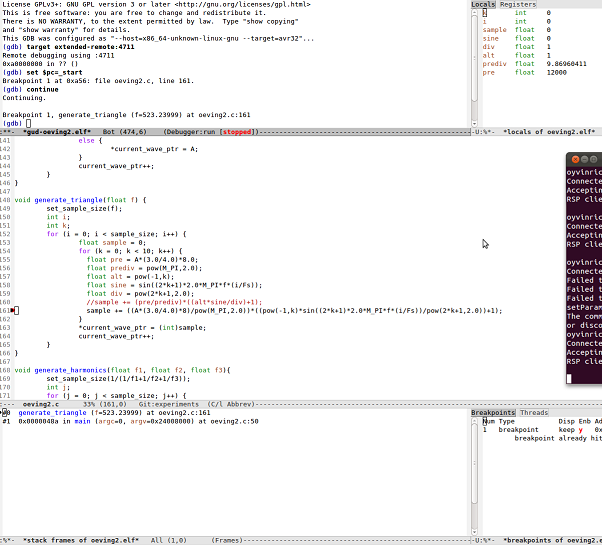
\includegraphics[scale=1]{images/debugsmall.png}
\end{center}

\section{Results}
The result of the exercise is that we coded a single program in C which generates and plays four different sounds when different switches (\emph{SW7} to \emph{SW4}) are pressed. At the start of the program it generates tones (\emph{A4} to \emph{C7}) based on the sine and triangle waves. Then once it gets an interrupt from a switch it plays the first sample of that switch whereafter the ABDAC generates an interrupt which plays the next sample until it is finished.

\section{Tests}
\paragraph{Description}
We've created a few test scenarios in order to test different aspects and corner cases of our code. The main prerequisites were the STK1000 development board, JTAGICE MKII and a headset.

The setup of the board: 
The headset was connected to the minijack on the development board, the jumper 4 and 5 was set to ''INT. DAC''.
Switches were connected to port C on the parallel I/O, and LED's on port B. 
Both the STK1000 and JTAGICE MKII debugger were connected and powered on. The tests were conducted by a person interacting with the switches wearing a headset, and another person logging the results.

\paragraph{Results}
Below is a table of the different tests we ran, the preconditions and the results.
\linebreak

\renewcommand{\arraystretch}{1.25} %vertical cell padding
\begin{tabular}[pos]{|m{70pt}|m{90pt}|m{90pt}|m{100pt}|m{60pt}|}
\hline
\textbf{Name} 				& \textbf{Preconditions}				& \textbf{Description} 					& \textbf{Expected result} 													& \textbf{Test result} 		\\ \hline

Steady-state test			& Power is on, and the board is connected & Upload program to card, push reset switch 	& The board is powered and LED 7 should be on 									& Passed 				\\ \hline

Move LED right test			& Program is active, only LED 7 is on 		& Push switch 6						 	& LED 7 should be turned off and LED 6 should be turned on 							& Passed 				\\ \hline

Move LED left test			& Program is active, only LED 6 is on 		& Push switch 7						 	& LED 6 should be turned off and LED 7 should be turned on 							& Passed 				\\ \hline

Left LED wrap-around test		& Program is active, only LED 7 is on 		& Push switch 67					 	& LED 7 should be turned off and LED 0 should be turned on 							& Passed 				\\ \hline

Right LED wrap-around test	& Program is active, only LED 0 is on 		& Push switch 6						 	& LED 0 should be turned off and LED 7 should be turned on 							& Passed 				\\ \hline

Long push test				& Program is active, only LED 7 is on 		& Push and hold switch 6 for a few seconds 	& LED 7 should be turned off and LED 6 should be turned on as soon as the switch is pushed 	& Passed 				\\ \hline
\end{tabular}

\section{Evaluation of assignment}
This assignment was more demanding yet also more fun than the first assignment. The learning curve was a bit harder as not all of us had coded much in C before, but it was a nice opportunity to learn.

\section{Conclusion}
We learned how to generate and play different sounds in C. This will be helpful when we start coding the next assignment. In the end we have four different sounds. Three short sound effects and one longer intro sound.

\section{Appendix}

\footnotesize{  % This makes the Reference items print in footnotesize fonts
\begin{thebibliography}{N}

\bibitem[1]{secure} AVR32 Architecture Document
\url{http://www.atmel.com/images/doc32000.pdf}

\bibitem[2]{secure} AT32AP7000 Datasheet
\url{http://www.atmel.com/Images/doc32003.pdf}

\bibitem[3]{secure} TDT4258 Compendium
\url{http://www.idi.ntnu.no/emner/tdt4258/_media/kompendium.pdf}

\end{thebibliography}  
}

\end{document} 
